%!TEX root = ../template.tex
%%%%%%%%%%%%%%%%%%%%%%%%%%%%%%%%%%%%%%%%%%%%%%%%%%%%%%%%%%%%%%%%%%%%
%% benchmark.tex
%% NOVA thesis document file
%%
%% Chapter with a short latex tutorial and examples
%%%%%%%%%%%%%%%%%%%%%%%%%%%%%%%%%%%%%%%%%%%%%%%%%%%%%%%%%%%%%%%%%%%%

\typeout{NT FILE benchmark.tex}

\chapter{Benchmark}
\label{cha:benchmark}

In this chapter, we present the third contribution from this dissertation, named ``PouchBeasts'' .PouchBeasts consists in a benchmark application for a back-end of an edge-enabled interactive multiplayer game, with functionality inspired from the popular game PokemonGO \todo{cite}. This contribution arose from the suggestion presented in \todo{cite this https://www.semanticscholar.org/paper/Towards-Enabling-Novel-Edge-Enabled-Applications-Leitao-Costa/7379b13c29b1543ef67adb969b08c9169836e750}, and aims to present a materialization of a benchmark with focus on real-time interactions between users. The importance of this contribution is its' possible use in testing service deployment systems, as the user interaction can be dramatically influenced in terms of quality of service as a function of the proximity of the deployment of its' services (i.e. users performing real-time battles mediated by a server in a different continent will have a poor user experience).

% PouchBeasts was attained through the combined efforts with a colleague, with the goal of being a proof-of-concept for the realization of a fully decentralized resource management system, that uses DeMMon as the solution for managing the nodes in an overlay network, and monitoring the execution of the PouchBeasts microservices. Then, this monitoring information is used by a decentralized service deployment solution to optimize the services supporting the execution of ``PouchBeasts'' via geographical heuristics (the latter is my colleagues' work).

PouchBeasts was attained through the combined efforts with a colleague, with the goal of being a proof-of-concept for the realization of a fully decentralized resource management system. The intention is to use this benchmark with DeMMon as the solution for managing the nodes in an overlay network, and for monitoring the execution of the PouchBeasts microservices. Then, this monitoring information is used by a decentralized service deployment solution to optimize the services supporting the execution of ``PouchBeasts'', via geographical heuristics, being the latter my colleagues' work.

In this application, registered users own a set of beasts, which they can expand by catching more beasts in certain gepgraphical areas, or by acquiring new ones in a shop. Beasts are collectable items with different properties (such as attack value, health points, experience, among other properties) which may be used to both battle against other users (and their beasts)and join other users in a cooperative battle against a computer-controlled beast. During these battles, users must command their beasts to either attack or defend and can also use items on their beasts, which can have multiple effects, such as: reviving dead beasts, healing a certain amount of health of a beat, among other uses. These items may be traded with other users or acquired from a shop using coins, which in turn are acquired through microtransactions.

\subsection{Overview}

\begin{figure}[htbp]
    \centering
    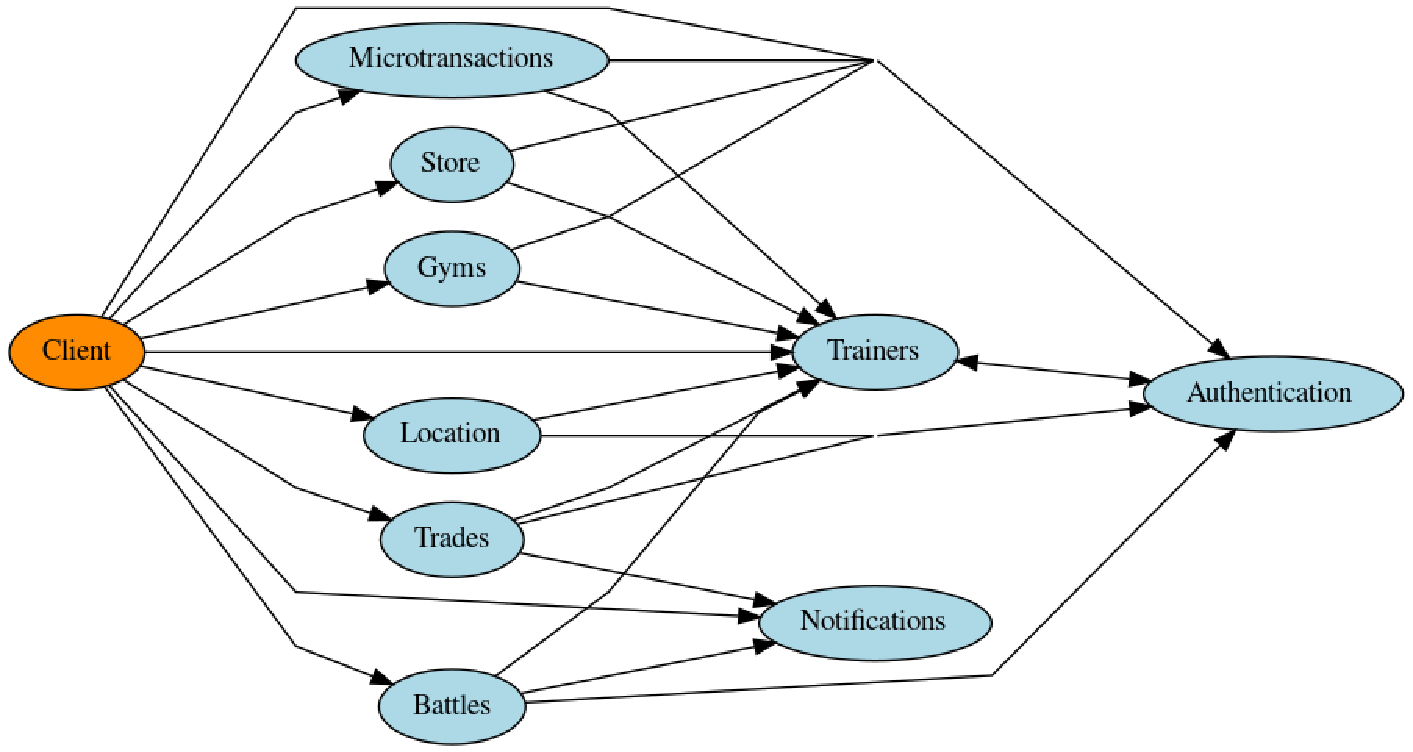
\includegraphics[width=\textwidth]{Chapters/benchmark/figures/interaction-diagram.pdf}
    \caption{An overview of the architecture of PouchBeasts}
    \label{fig:pouchbeasts-overview}
\end{figure}

The interactions between the services in this benchmark are illustrated in the diagram of figure \ref{fig:pouchbeasts-overview}. There are nine microservices in total and a client to access them. We now provide a brief overview of each microservice and its role within the system:

\begin{enumerate}
    \item The first and most used microservice of the system is called \textbf{Trainers} and it essentially stores all the data related to the users and their owned beasts. In addition, the service verifies the tokens issued by the authentication microservice in regards to the recency of the information carried in the token. This service makes use of a MongoDB \todo{cite} database to store these records in a permanent storage and to maintain data consistency across microservices.
    
    \item The next microservice is called \textbf{Authentication}, which only has the purpose of generating new authentication tokens for the users to use when interacting with other services. These tokens contain a hash of the owned beasts, so other servers can verify their authenticity and recency without having to fetch the users' beasts on each interaction.

    \item Following, we have the \textbf{Gyms} and \textbf{Battles} services and these allow players to perform combats with their obtained beasts. In the case of the gym's service, it manages entities in the system denominated gymnasiums, which have a pre-assigned geographical location. In this service, if a user is within a geographical distance of a gymnasium, it may perform battles alongside other trainers against a single beast controlled by the computer. The \textbf{Battles} service is a service that allows users to use their beasts to perform battles against other users' beasts. Battles can either start via a queueing system, where players wait for another random user to start the battle, or alternatively via challenging other known users (via a notification). As previously mentioned, whenever a user is in a battle, it issues moves (based on the observed battle status) and receives updates regarding the status of the battle. As moves depend on the observed status of the battle, it is paramount (for the quality of service of the users) that both the moves of the players and the information passed from the battles/gyms service to the player suffers the least latency possible. The information regarding the issued and the status of battle is propagated to the user using WebSockets. Whenever the battle is finished, the Battles / Gyms server commits the battle result and update the users' beasts in the Trainers service.
    
    \item The \textbf{Store} and \textbf{Microtransactions} services provide ways for users to obtain currency via small value transactions, which can, in turn, be used in the store to buy new items. These items then have effects on the beasts (e.g. or reviving a dead beast or healing a beast which has little health).

    \item Users may also change their items via the \textbf{Trades} service, this service grants users the possibility to exchange their items with other users in the system. In order to use this system, a user must invite another currently active user via a notification (which can optionally be accepted by the target user). Whenever this notification is accepted, the two users connect to the server via a websockets connection and begin to submit to the services the items they wish to be traded with the other user. Whenever a player adds an item to the trade, this information is propagated by the server to the other player through a WebSockets connection. Whenever the users are finished adding or removing items to be traded, they accept the trade, and the transaction result is submitted to the trainers server.

    \item The service responsible for handling all of the previously mentioned notifications is called \textbf{Notifications}. This service is essentially tasked with receiving notifications from connected users and propagating them towards the target user. As there may be multiple notification services executing concurrently and users may connect to any of the available servers, a notification may be emitted for a user not connected to the same server. To prevent these notifications from being lost, this service makes use of a Kafka backend, which it uses to propagate messages for nodes that are connected to different notification servers.

    \item The last implemented microservice is called \textbf{Location} service, this service is responsible for managing the geographical locations of the users using the system, the generation and management of the generated beasts (for users to catch), and the locations of gymnasiums in a certain geographical area. Propagation of this information is done in a periodic manner via a WebSockets API. In order to prevent multiple location services from managing overlapping geographical areas, and to facilitate the insertion and decommission of new location servers, we assign portions of the geographical area to certain servers using S2 cells \todo{cite}. S2 cells provide a framework for decomposing a sphere (in our case, the earth) into a hierarchy of cells, where each S2 cell is quadrilateral bounded by four geodesics. The top-level of the hierarchy is obtained by projecting the six faces of a cube onto the earth, and lower levels are obtained by subdividing each cell into four children recursively. An example of two of the six face cells (one of which has been subdivided multiple times) can be observed in figure \ref{fig:pouchbeasts-s2cells}, obtained from \todo{cite}. This service makes use of S2 cells to (1) assign portions of the earth to servers in a way that does not create geographical discontinuities, (2) to index efficiently the locations of trainers, gyms and generated beasts, which allows the service to, based on cell centred on a user-provided location, determine the beasts and gyms to return to the user, (3) in the case a user's location is in the boundary of two (or more) location servers, S2 cells are also used to decide to which server(s) the user should connect to, so that it does not receive only a portion of the results for its correspondent geographical area, and finally (4) to allow a dynamic subdivision and collapse of geographical regions to instantiate or decommission location servers.
\end{enumerate}

\begin{figure}[htbp]
    \centering
    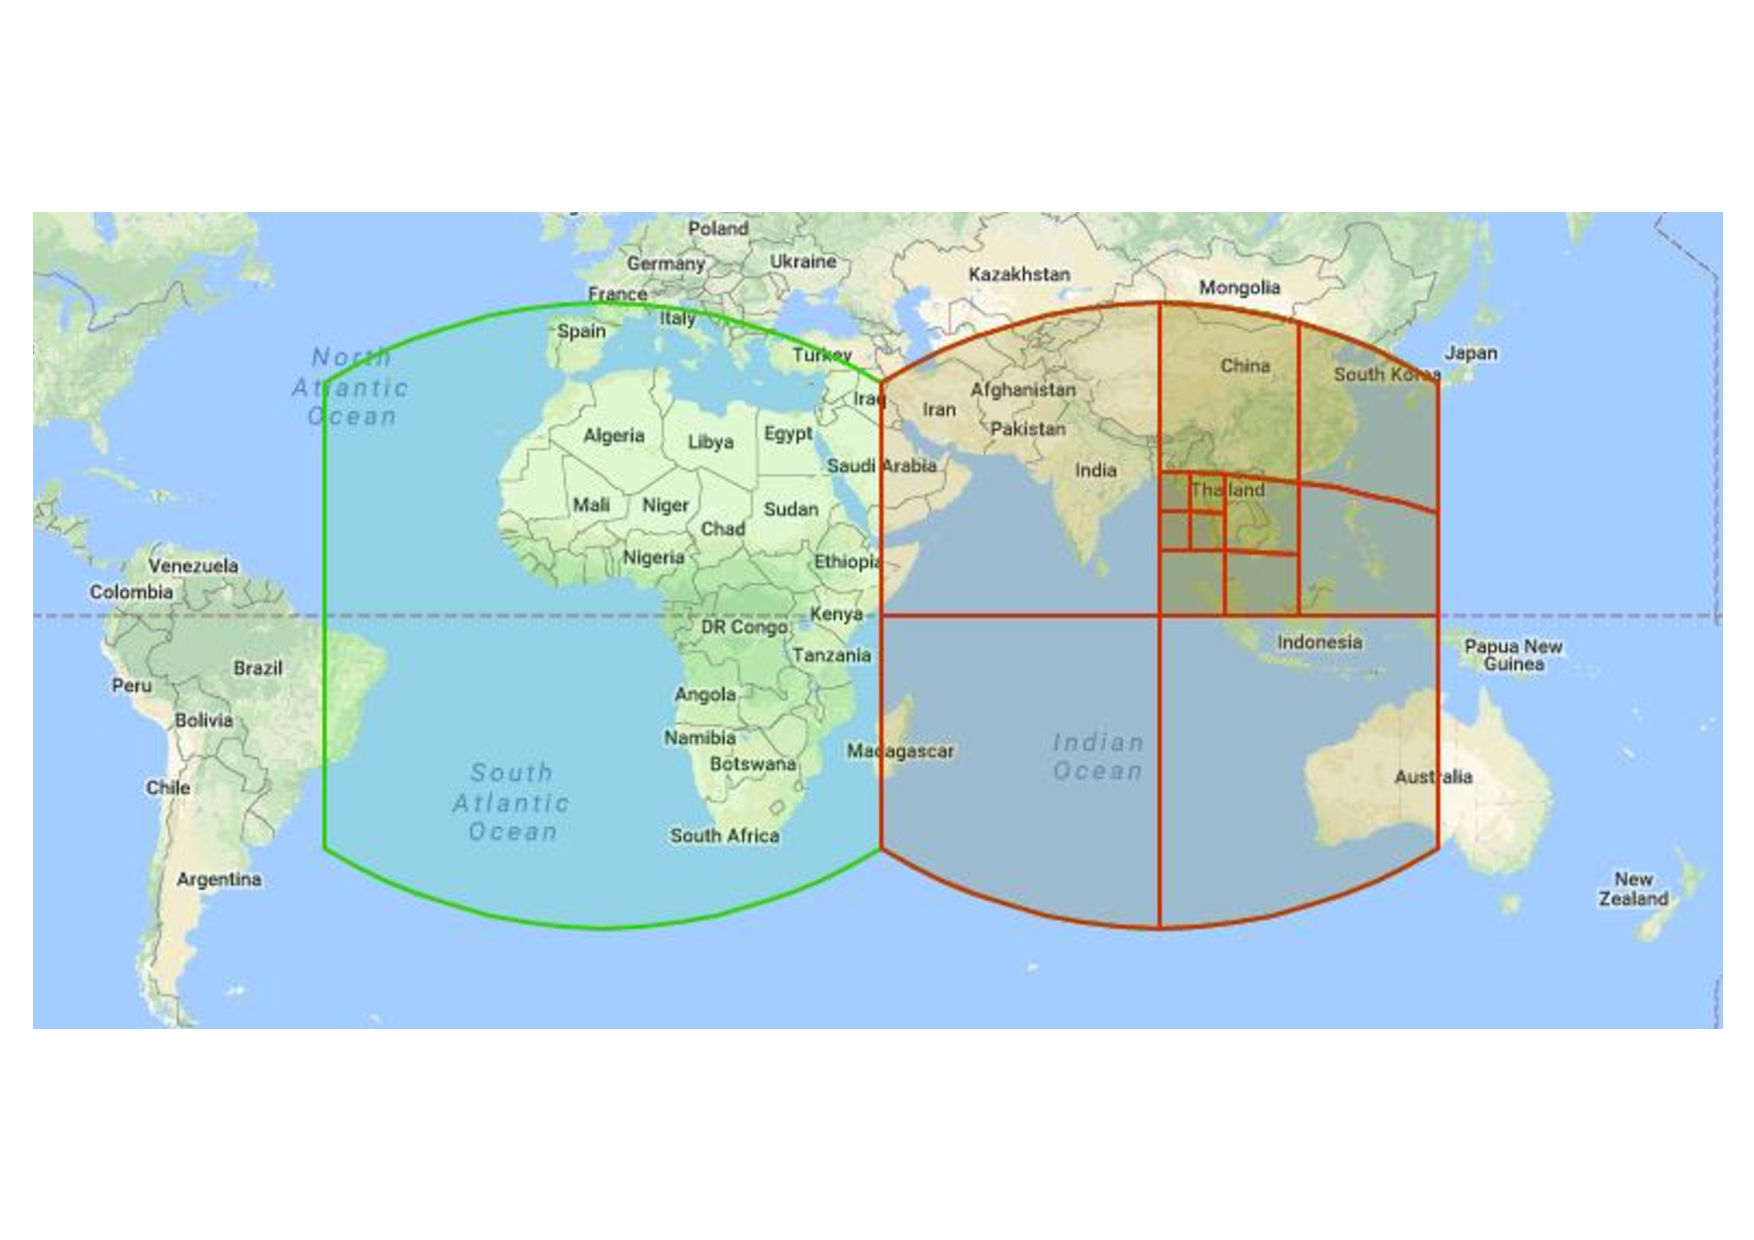
\includegraphics[width=\textwidth]{Chapters/benchmark/figures/s2_cells.pdf}
    \caption{Example of S2 cell hierarchy}
    \label{fig:pouchbeasts-s2cells}
\end{figure}

Provided with the high-level overview of each of the implemented microservices of the benchmark, it is important to notice that the latency requirements regarding the interactions with the users and services are varied. For example, services such as the Trainers, Store or Microtransactions services are more tolerant when it comes to latency requirements when compared to services like the Gyms, Battles or Trades, as these have an interactive nature where a high latency value leads to frustration when it comes to user experience (i.e. having a delay in a battle may cause a certain users to lose in a way which feels unfair).

To enable this experimentation of these interactions, the benchmark also contains a client which allows the execution of actions such as: battling other users, catching beasts, acquiring and spending tokens, among others actions. Then, through the instrumentation of both the client and the services, we provide a way to quantify some aspects regarding these interactions, such as the delays in the interactions between users and servers in both trades and battles services, among other interactions. Provided with these indicators, users may then acess the performance of their service deployment and maintenance systems.

To enable automated client testing, we provide ways for client to simulate user behavior. This behavior is configurable via a configurable stochastic matrix \todo{cite this from somwhere else other than wikipedia https://en.wikipedia.org/wiki/Stochastic\_matrix}. This matrix contains a line and a row for each possible action to perform with the client, and each matrix position (provided by a certain line and row) contains the probability of performing any of the other possible actions, provided the user just performed the action in the current line. 

\subsection{Summary}

In this chapter, we covered the third contribution from this dissertation, named ``PouchBeasts''. This contribution, in the shape of a benchmark, aims to simplify the evaluation process of decentralized management and monitoring solutions, particularly those aimed at improving service deployments. It does so by providing both a client and a set of services (implemented by microservices) which offer a wide range of interaction types, from request-reply based interactions to real-time interactions which have varied demands in regard to server and client latency.

Although this benchmark was not employed to test the performance of DeMMon directly, it is important to mention that the colleague that was contributing in the implementation of this benchmark has successfully built a system (for his own dissertation) that, through the metrics obtained by the DeMMon framework, improves the QOS of clients using the ``PouchBeasts'' services.